\chapter{Solution}
\minitoc


* Terminology: The item is now a product, and the user is now a customer of an e-commerce platform

\section{System Components}


!!! TODO say we will build the "custom Ops" in the following graph

TODO maybe we have to create our own custom graph to add caching, API gateway, and automation and DevOps components with our own infrastructure 

\begin{figure}[H]
    \centering
    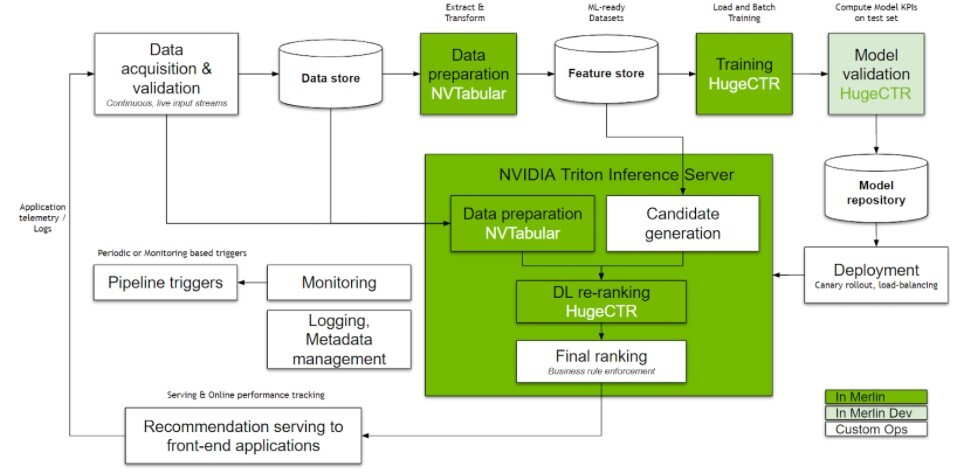
\includegraphics[width=1\textwidth]{assets/components.jpeg}
    \caption[System Components]{System Components \cite{NvidiaRecSysBestPractices}}
\end{figure}



* API gateway
    * data ingestion
    * adding new customers, items, and interaction endpoints 
    * getting recommendations for a customer endpoint [ and how it first queries the caching layer and then the recommendation pipeline]
* Recommendation Pipeline ( all the stages )
    * Retrieval
    * Filtering
    * Scoring
    * Ordering
* Caching Layer
* Automation and DevOps
* Components Deployment ( ECS or Kubernetes, SageMaker or Triton Inference Server, Redis or Memcached, which feature store )?



\section{Candidate Generation}




\subsection{Two Tower Model (Retrieval)}
* embedding store?
* choosing a ranking model and explaining it

\subsection{Bloom Filte (Filtering)}
* Explaining the E-commerce business logic
TODO 



\subsection{Deep Learning Ranking Model (Scoring Stage)}

* feature store 
* choosing a ranking model and explaining it
* storing model parameters?


TODO

\subsection{E-commerce ordering logic (Ordering Stage)}

* add additional business logic like promoting items (sponsored items), write an equation for the final score ( maybe ranking score + 0.2 for sponsored items or put sponsored items on top of the list if they exceed a certain threshold score)

TODO

\subsection{Storing Results (Caching Layer)}

* Redis or any memory store

TODO

\subsection{Deployment of components ?}
